% =====================================================================
%  Blog post template: compiles in Overleaf AND builds on the website.
%
%  Overleaf:  New Project -> Upload Project -> overleaf-post.zip
%             (main document = index.tex, compiler = pdfLaTeX)
%  Publish:   Overleaf Menu -> Download -> Source (.zip), unzip into
%             posts/<yyyy-mm-short-name>/ in the blog repo, edit meta.yaml,
%             then git add / commit / push.
%
%  Rules that keep both outputs working:
%   * Title, date, category, summary live in meta.yaml (not \title/abstract;
%     the website ignores those).
%   * Figures: PNG/JPG/PDF in figs/, referenced as figs/<name>.
%   * Define macros with \providecommand (the site also defines them).
%   * Number equations with \label{eq:...} and cite them with \eqref{...}.
% =====================================================================
\documentclass[11pt]{article}
\usepackage[margin=2.5cm]{geometry}
\usepackage{amsmath, amssymb}
\usepackage{graphicx}
\usepackage{listings}
\usepackage{xcolor}
\usepackage{hyperref}
\lstset{basicstyle=\ttfamily\small, columns=fullflexible, frame=single, breaklines=true}

% Shared site macros (same as macros.tex in the blog repo)
\providecommand{\dd}{\mathrm{d}}
\providecommand{\dv}[2]{\frac{\mathrm{d}#1}{\mathrm{d}#2}}
\providecommand{\pdv}[2]{\frac{\partial #1}{\partial #2}}
\providecommand{\tr}{\operatorname{tr}}

% Shown only in the PDF; the website uses meta.yaml
\title{The Damped Harmonic Oscillator}
\author{Sodtavilan Odonchimed}
\date{}

\begin{document}
\maketitle

The opening paragraph appears on the website right after the table of contents.
Inline math works as usual, for example $\omega_0 = \sqrt{k/m}$.

\section{Equation of motion}\label{sec:eom}

A mass $m$ on a spring of stiffness $k$ with linear damping $c$ obeys
\begin{equation}\label{eq:eom}
  m \dv{^2x}{t^2} + c \dv{x}{t} + k x = 0 .
\end{equation}
Dividing by $m$ and writing $\gamma = c / 2m$ gives the standard form
\cite{goldstein2002}:
\begin{align}
  \ddot{x} + 2\gamma \dot{x} + \omega_0^2 x &= 0, \label{eq:standard} \\
  \omega_0^2 &= k / m . \nonumber
\end{align}

\section{Solution}\label{sec:solution}

For weak damping ($\gamma < \omega_0$) the solution of Eq.~\eqref{eq:standard} is
\begin{equation}\label{eq:solution}
  x(t) = A\, e^{-\gamma t} \cos(\omega_d t + \varphi),
  \qquad \omega_d = \sqrt{\omega_0^2 - \gamma^2},
\end{equation}
shown in Figure~\ref{fig:damped}. Section~\ref{sec:eom} has the derivation.

\begin{figure}[ht]
  \centering
  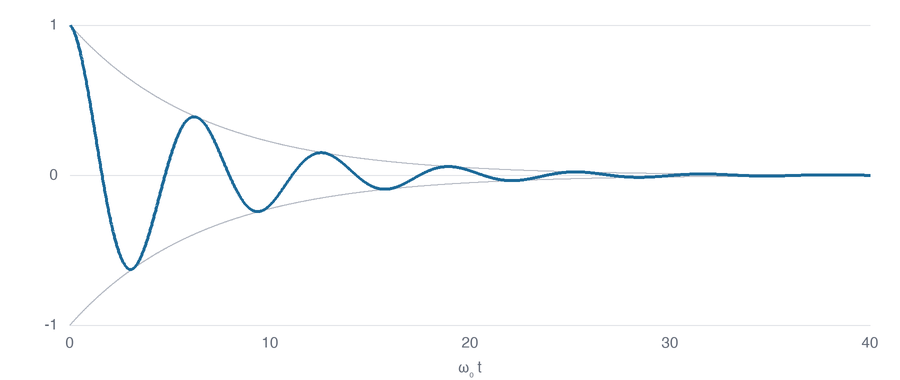
\includegraphics[width=0.8\linewidth]{figs/damped.png}
  \caption{Displacement $x(t)$ from Eq.~\eqref{eq:solution} with
  $\gamma = 0.15\,\omega_0$.}
  \label{fig:damped}
\end{figure}

\begin{table}[ht]
  \centering
  \begin{tabular}{lll}
    Regime & Condition & Behaviour \\
    Underdamped & $\gamma < \omega_0$ & decaying oscillation \\
    Critical & $\gamma = \omega_0$ & fastest return, no overshoot \\
    Overdamped & $\gamma > \omega_0$ & slow return, no oscillation \\
  \end{tabular}
\end{table}

\section{Simulation}

\begin{lstlisting}[language=Python]
import numpy as np

def damped(t, omega0=1.0, gamma=0.15, A=1.0, phi=0.0):
    omega_d = np.sqrt(omega0**2 - gamma**2)
    return A * np.exp(-gamma * t) * np.cos(omega_d * t + phi)

t = np.linspace(0, 40, 2000)
x = damped(t)
\end{lstlisting}

\bibliographystyle{plain}
\bibliography{refs}

\end{document}
